\NeedsTeXFormat{LaTeX2e}
\documentclass[a4paper,12pt,
headsepline,           % Linie zw. Kopfzeile und Text
oneside,               % einseitig
pointlessnumbers,      % keine Punkte nach den letzten Ziffern in Überschriften
bibtotoc,              % LV im IV 
%DIV=15,               % Satzspiegel auf 15er Raster, schmalere Ränder   
BCOR15mm               % Bindekorrektur
%,draft
]{scrbook}
\KOMAoptions{DIV=last} % Neuberechnung Satzspiegel nach Laden von Paket helvet
\KOMAoption{listof}{totoc} % AV im IV

\pagestyle{headings}
\usepackage{blindtext}

% für Texte in deutscher Sprache
\usepackage[T1]{fontenc}      % sollte immer das erste der drei Pakete sein!
\usepackage[ngerman]{babel}
\usepackage[utf8]{inputenc}

% Helvetica als Standard-Dokumentschrift
\usepackage[scaled]{helvet}
\renewcommand{\familydefault}{\sfdefault} 

% für Bilder
\usepackage{graphicx}
\usepackage{caption}
\usepackage{subcaption}
\usepackage{wrapfig} % Bild mit Textumfluss
\counterwithout{figure}{chapter} % für durchgehende Nummerierung

% Literaturverzeichnis mit BibLaTeX
\usepackage[babel,german=quotes]{csquotes}
\usepackage[backend=biber,style=verbose-ibid]{biblatex}
\addbibresource{meine-literatur-22.bib}
\DefineBibliographyStrings{german}{
    editor    = {Hg\adddot}
}

%Für Tabellen
\usepackage{longtable}
\usepackage{booktabs}

% Besondere Schriftauszeichnungen
\usepackage{url}              % \url{http://...} in Schreibmaschinenschrift
\usepackage{color}            % zum Setzen farbigen Textes

\usepackage{amssymb, amsmath} % Pakete für Mathe-Umgebungen und -Symbole

\usepackage{setspace}         % Paket für div. Abstände, z.B. ZA
%\onehalfspacing              % nur dann, wenn gefordert; ist sehr groß!!
\setlength{\parindent}{0pt}   % kein linker Einzug der ersten Absatzzeile
\setlength{\parskip}{1.4ex plus 0.35ex minus 0.3ex} % Absatzabstand, leicht variabel

% Tiefe, bis zu der Überschriften in das Inhaltsverzeichnis kommen
\setcounter{tocdepth}{3}      % ist Standard

% Renaming der Caption
\captionsetup{
  figurename=Bild,
  labelfont=bf,
  font={footnotesize,sf}
}
\renewcommand{\thefigure}{\textbf{\arabic{figure}}}

%Verwesie
\usepackage{varioref}
\usepackage{hyperref}
\usepackage[german]{cleveref}
\crefname{section}{}{}

% Beispiele für Quellcode
\usepackage{listings}
\lstset{language=Java,
  showstringspaces=false,
  frame=single,
  numbers=left,
  basicstyle=\ttfamily,
  numberstyle=\tiny}

% hier Namen etc. einsetzen
\newcommand{\fullname}{Maximilian Hauser}
\newcommand{\email}{maximilian.hauser@uni-ulm.de}
\newcommand{\titel}{LaTeX - praktische Anwendung in wissenschaftlichen Arbeiten}
\newcommand{\jahr}{2022}
\newcommand{\matnr}{1096838}
\newcommand{\gutachterA}{Prof.\,Dr.\,Streng Geheim}
\newcommand{\gutachterB}{Prof.\,Dr.\,Un Leserlich}
\newcommand{\betreuer}{Betreuername}

% hier die Fakultät auswählen
%\newcommand{\fakultaet}{***  Fakultät im LaTeX-Quellcode anpassen nicht vergessen! ***}
\newcommand{\fakultaet}{Ingenieurwissenschaften, Informatik und Psychologie}
%\newcommand{\fakultaet}{Mathematik und\\Wirtschafts-\\wissenschaften}
%\newcommand{\fakultaet}{Medizin}
%\newcommand{\fakultaet}{Naturwissenschaften}

% hier das Institut einsetzen
\newcommand{\institut}{Medieninformatik B.Sc.}

% Informationen, die LaTeX in die PDF-Datei schreibt
\pdfinfo{
  /Author (\fullname)
  /Title (\titel)
  /Producer     (pdfeTex 3.14159-1.30.6-2.2)
  /Keywords ()
}

\usepackage{hyperref}
\hypersetup{
pdftitle=\titel,
pdfauthor=\fullname,
pdfsubject={Diplomarbeit},
pdfproducer={pdfeTex 3.14159-1.30.6-2.2},
colorlinks=false,
pdfborder=0 0 0	% keine Box um die Links!
}

% Trennungsregeln
\hyphenation{Sil-ben-trenn-ung}

\begin{document}
\frontmatter

% Titelseite
\thispagestyle{empty}
\begin{addmargin*}[4mm]{-10mm}

\hfill

\includegraphics[height=1.8cm]{rohmaterial-bilder/Logo_uulm_Vorlage_100mm_schwarz.pdf}\\[-1.25em]

{\footnotesize
%{\bfseries Universität Ulm} \textbar ~89069 Ulm \textbar ~Germany
\hspace*{115mm}\parbox[t]{35mm}{\bfseries Fakultät für\\
\fakultaet\\
% TODO hier Institut anpassen
\mdseries \institut}\\[2cm]

\parbox{140mm}{\bfseries \LARGE \titel}\\[2.5em]
{\bfseries \LARGE Hausarbeit als Leistungsnachweis}\\[5em]

{\footnotesize \bfseries Vorgelegt von:}\\
{\footnotesize \fullname\\ \email}\\ \\[2em]
}
\end{addmargin*}


% Impressum
\clearpage
\thispagestyle{empty}
{ \small
  \flushleft
  Fassung \today \\\vfill
  \copyright~\fullname\\[0.5em]
% Wenn Sie Ihre Arbeit unter einer freien Lizenz bereitstellen möchten, können Sie die nächste Zeile in Ihren Code aufnehmen. Bitte beachten Sie, dass Sie hierfür an allen Inhalten, inklusive enthaltener Abbildungen, die notwendigen Rechte benötigen! Beim Veröffentlichungsexemplar Ihrer Dissertation achten Sie bitte darauf, dass der Lizenztext nicht den Angaben in den Metadaten der genutzten Publikationsplattform widerspricht. Nähere Information zu den Creative Commons Lizenzen erhalten Sie hier: https://creativecommons.org/licenses/
This work is licensed under the Creative Commons Attribution 4.0 International (CC BY 4.0) License. To view a copy of this license, visit \href{https://creativecommons.org/licenses/by/4.0/}{https://creativecommons.org/licenses/by/4.0/} or send a letter to Creative Commons, 543 Howard Street, 5th Floor, San Francisco, California, 94105, USA. \\
  Satz: PDF-\LaTeXe
}

% ab hier wird Zeilenabstand etwas größer gesetzt
\setstretch{1.1}

\tableofcontents

\mainmatter
Lehre und Lernen 4.0: Zwischen Tafel und Tablet

Lehre gut, alles gut!

Im deutschen Wissenschaftsbetrieb zog die Lehre lange Zeit den Kürzeren. Zwar steht sie noch immer im Schatten der Forschung, aber in der Politik und an den Universitäten tut sich was. Bund-Länder Programme wie der „Qualitätspakt Lehre“ setzen dabei deutliche Signale und haben an vielen Hochschuleinrichtungen das Thema Lehre zur Chefsache befördert. An der Universität Ulm kümmert sich das Zentrum für Lehrentwicklung (ZLE) um all diejenigen, die in der Lehre an vorderster Front stehen.

Lehre kann sehr beglückend sein: wenn man vorne im Hörsaal steht und sprichwörtlich hören kann, wie bei den Zuhörern der Groschen gefallen ist, wenn es gelingt, die Studierenden im Gedankenstrom mitzureißen und zu begeistern. Es kann aber auch frustrieren, wenn man merkt, kaum einer passt auf. Umso wichtiger ist es, die Lehrenden bei ihrer Arbeit professionell zu unterstützen. „Gute Lehre ist nicht nur entscheidend für die erfolgreiche Vermittlung von Wissen. Sie weckt Begeisterung für das Fach und motiviert für die Auseinandersetzung mit wissenschaftlichen Fragen. Auch die Forschung braucht gute Lehre“, erklärt Professorin Irene Bouw. Die Vizepräsidentin für Lehre und Internationales leitet das 2017 geschaffene Zentrum für Lehrentwicklung (ZLE), das als Stabsstelle dem Präsidium der Universität Ulm zugeordnet ist. Dort finden die Bereiche Hochschuldidaktik, E-Learning und Lehrerbildung eine neue Heimat.

% Einbinden von zwei Abbildungen nebeneinander mit je einer eigenen Beschriftung sowie einer gemeinsamen Bildunterschrift

Gegründet wurde das ZLE, um alle fachübergreifenden Programme und Aktivitäten zur Lehre zu bündeln und zentral zu steuern. Aufgehängt sind dort auch die erfolgreichen Drittmittelprojekte „UULM PRO MINT \& MED“ oder „PASSt!“, die den Studieneinstieg erleichtern und größere individuelle Spielräume für Studierende schaffen sollen. Das übergeordnete Ziel: insbesondere in den technisch-naturwissenschaftlichen Fächern den Studienerfolg verbessern und Abbrecherquoten senken. Dauerhafte Strukturen sollen nun dabei helfen, Projekterfolge zu verstetigen und vielversprechende Maßnahmen fortzuführen. 

Von der Arbeit des Zentrums für Lehrentwicklung profitieren Professorinnen und Professoren gleichermaßen wie Lehrende aus dem Mittelbau oder Doktoranden und Studierende. Ob mit Workshops, individuellen Beratungen oder Hospitationen: Angebote und didaktisches Knowhow sind passgenau zugeschnitten auf die jeweilige Lehrsituation und den persönlichen Bedarf. 

[\ldots]

Digitale Medien in der Lehre

Neue Möglichkeiten für die Lehre bietet der Einsatz von digitalen Lehr- und Lernmitteln. Hier hilft die Abteilung E-Learning. In Kooperation mit dem  Kommunikations- und Informationszentrum der Uni (kiz) unterstützen die ZLE-Mitarbeiter Lehrkräfte, wenn es darum geht, Inhalte und Formate für die digitalisierte Lehre zu erstellen. Während digitale Lernplattformen wie MOODLE an der Uni Ulm bereits fester Bestandteil der Lehre sind, spielen sogenannte Onlinevorlesungen wie MOOCS (Massive Open Online Courses) keine Rolle. „Digitale Medien können die Lehrenden nicht ersetzen. Die Universität Ulm versteht sich als Präsenzuniversität!“, betont die Leiterin der Abteilung E-Learning am ZLE, Dr. Tatjana Spaeth. In der Regel geht es in den Workshops und individuellen Beratungsgesprächen des Zentrums daher eher um so genannte Blended Learning Formate, also die Verbindung von Präsenz- und Onlineelementen in der Lehre sowie um die didaktisch-praktische Unterstützung bei der Vor- und Nachbereitung von Lehrveranstaltungen. Die E-Learning-Experten leisten beispielsweise Hilfestellung beim Umgang mit der Onlineplattform MOODLE, mit deren Hilfe nicht nur Lehrmaterialen bereitgestellt und Veranstaltungen evaluiert werden, sondern auch die Kommunikation zwischen Dozent und Kursteilnehmern organisiert ist. Fragen zu Nutzungsrechten oder zum Urheberrecht klärt das E-Learning-Team in Zusammenarbeit mit den entsprechenden Stellen an der Uni; beispielsweise mit den Juristen aus dem Dezernat I der Zentralen Universitätsverwaltung oder mit den kiz-Mitarbeitern aus dem Bereich „Wissenschaftliche Informationsdienste“. Grundsätzlich gilt für den Einsatz digitaler Medien: Das Neue ist nicht immer besser. „E-Learning macht das Lernen nicht unbedingt leichter. Es erfordert ein hohes Maß an Eigenverantwortung“, gibt die Psychologin Spaeth zu bedenken. Und auch das Lehrbuch wird dadurch sicherlich nicht aussterben. 

[\ldots]

Gute Lehre macht Schule! 

Die Universität Ulm ist eine MINT-Uni mit einem starken naturwissenschaftlich-technischen Profil. Mit der Lehrerbildung in Fächern wie Chemie, Biologie und Physik sowie Informatik, Mathematik und Wirtschaftswissenschaften übernimmt sie gesellschaftliche Verantwortung, um junge Menschen für Fächer zu begeistern, die für die wirtschaftliche und technologische Zukunftsfähigkeit des Landes entscheidend sind. Die Abteilung Lehrerbildung am ZLE ist an der Uni die zentrale Anlaufstelle für alle Lehramtsstudierenden. In Zusammenarbeit mit den jeweiligen Fachbereichen können sich dort angehende Lehrerinnen und Lehrer bei der Planung und Organisation ihres Studiums beraten und unterstützen lassen. Von dort aus laufen die Fäden zum Landeslehrerprüfungsamt, zum Kultusministerium, den Ausbildungsschulen und den Seminaren für Didaktik und Lehrerbildung. „Denn erfolgreich unterrichten können nur Lehrer, die sowohl fachlich als auch pädagogisch-didaktisch gut ausgebildet sind“, erklärt Marc Lamche, der am ZLE den Bereich Lehrerbildung leitet. 

% Einfügen eines Bilds in Textbreite mit Bildbeschriftung

Für alle, die sich intensiver mit Lehrthemen befassen, vom Dozenten bis zur Doktorandin, von der Professorin bis zum Student, gibt es einen Termin, den sie sich merken sollten. Beim „Tag der Lehre“, der Anfang Dezember zum ersten Mal stattfand und jetzt jährlich ausgetragen werden soll, können sich Interessierte bei den Didaktikexperten und Lehrforschern neue Ideen und Impulse für die Praxis holen. Denn gute Lehre geht über reine Vermittlung von Fachwissen weit hinaus. Sie ist ein wichtiges Instrument der Erkenntnis, die dabei helfen soll, kritisch zu denken und verantwortungsvoll zu handeln. Sinnvoll ist dabei alles, was nützt: damit der Groschen auch wirklich fällt! 


Fünf Tipps des ZLE für Lehrende

\ldots von Dr. Cornelia Estner

% Welche Umgebung für diese Art der Aufzählung?

\begin{???}
\item Die normale Aufmerksamkeitsspanne beträgt ca. 20-30 Minuten. Danach sollte
ein methodisch-didaktischer Wechsel stattfinden: Nach einem Frontalvortrag könnte z.B. ein 
Film gezeigt werden.
\item Im Laufe von Veranstaltungen bieten sich kurze „Lernstopps“ an: So erhalten die 
Zuhörerinnen und Zuhörer Gelegenheit, das Gehörte zu verarbeiten.
\item Bei einer semesterbegleitenden oder mehrtägigen Veranstaltung ist es sinnvoll, zum Einstieg immer eine kurze Wiederholung der letzten Einheit anzubieten – eventuell in Quizform. 
\item Zu Beginn jeder Lehrveranstaltung, egal ob wiederkehrend
oder einmalig, sollte ein Themenüberblick gegeben werden. Gut ist auch eine Darstellung der Lernziele („Am Ende der heutigen Einheit können Sie \ldots{}“).
\item Die Powerpoint-Präsentation einer Veranstaltung sollte nicht gleichzeitig das Skript
sein. Idealerweise enthalten die Vortragsfolien überwiegend Bilder oder maximal
acht Bullet-Points.
\end{???}

Der Abschnitt ** Querverweis auf Abschnitt Lehre gut, alles gut! ** sowie die Unterabschnitte ** Querverweis auf Unterabschnitt Digitale Medien in der Lehre ** bis ** Querverweis auf Unterabschnitt mit den 5 Tipps für Lehrende *** sind Auszüge aus *** Inline-Zitat aus uni ulm intern, Seiten 4 bis 7 ***. Wir danken der Pressestelle der Universität Ulm für die freundliche Genehmigung der Verwendung von Text und Bildern.

Lernen will gelernt sein! Interview mit Prof. Tina Seufert

Lernen, lernen, lernen: Viele Studierende fragen sich vor der Prüfungsphase, wie sie sich umfangreichen Stoff aneignen sollen. Professorin Tina Seufert ist Lehr-/Lernforscherin und weiß genau, worauf es im Hörsaal und am Schreibtisch ankommt. [\ldots]

Frau Prof. Seufert, gerade gegen Semesterende füllen sich die Bibliotheken und Lernflächen der Universität Ulm. Dabei scheint das Lernen einigen Studierenden deutlich leichter zu fallen als anderen. Wie funktioniert überhaupt erfolgreiches Lernen?

„Lernen ist die Auseinandersetzung beziehungsweise die Verarbeitung von Informationen. Sie sollen langfristig gespeichert und so abgelegt werden, dass sie wieder auffindbar sind. Gute Lerner beobachten sich selbst und reflektieren ihren Lernprozess: Was läuft gut beim Lernen? Die einfachsten Reaktionen darauf wären, bei Nichtverstehen nachzufragen oder die nicht verstandene Textpassage noch einmal zu lesen. Gutes Zeitmanagement gehört natürlich auch dazu, sowie die Fähigkeit, sich und die eigene Aufnahmefähigkeit einzuschätzen. Insgesamt wird man durch Selbstbeobachtung und -regulation zum erfolgreichen Lerner.“

Gibt es denn verschiedene Lerntypen, und wie findet man die für sich optimale Methode?

„In der Lehr-/Lernforschung sprechen wir inzwischen ungerne von Lerntypen wie dem Bild- oder Texttyp. Welches Vorgehen Erfolg verspricht, hängt eher vom Stoff ab. Beispielsweise sollten angehende Ingenieure, die sich mit Schaltkreisen beschäftigen, anders lernen als ein Historiker, der geschichtliche Zusammenhänge verstehen will. Auch hier ist die Selbstbeobachtung, von uns Forschern Metakognition genannt, wichtig: Das Lernverhalten sollte reflektiert und gegebenenfalls angepasst werden. In der Forschung gehen wir also eher von flexiblen Lernwegen als von Typen aus.“

Lern-Apps oder YouTube-Tutorials haben sicher alle Studierenden schon einmal genutzt. Inwiefern verändern digitale Medien das Lernen? Und welche Aspekte sind aus Forschersicht Fluch, welche Segen?

„Der eigentliche Lernprozess verändert sich durch digitale Medien nicht. Allerdings müssen Lernende bei ihrem Einsatz gegebenenfalls stärker unterstützt werden. Wer mit einer Lern-App arbeitet, gerät eventuell stärker in Versuchung, seine Mails zu checken oder nebenbei soziale Medien zu nutzen. Auf der anderen Seite bieten solche Apps auch neue Möglichkeiten: Studierende, die die in Ulm entwickelte Mikroskopie-App MyMi.Mobile einsetzen, können beispielsweise Präparate nutzen, die ihnen sonst nicht jederzeit zur Verfügung stehen. Gleiches gilt für Augmented Reality-Anwendungen und Simulationen, mit denen etwa Notfalleinsätze trainiert werden. Dabei darf man Fehler machen, was für das erfolgreiche Lernen wichtig ist. Ein weiterer Vorteil digitaler Medien: Sie sind für heutige Lerner attraktiv, allerdings wird in einigen Jahren ein Gewöhnungseffekt einsetzen.“

Lernen überall und zu jeder Zeit – zum Beispiel per App im Bus oder mit dem Tablet-PC auf dem Sofa – ist das überhaupt sinnvoll?

„Diese ständige Verfügbarkeit von Angeboten wird dem individuellen Lernen gerecht. An Universitäten wird die Studierendenschaft immer heterogener und bei den Lernvoraussetzungen ergeben sich hieraus große Unterschiede. Dem trägt eine stets verfügbare Lern-App, mit der Inhalte individuell und zeitunabhängig vertieft werden, Rechnung. Generell ist es gut, das Lernen in den Alltag zu integrieren und zum Beispiel ein Lernpropramm auch mal im Café zu nutzen. Dabei sollte der Lerner natürlich sich selbst und die eigenen Konzentration beobachten.“

Vom Lernen zur Lehre: Was macht für Sie als Forscherin gute Lehre aus?

„Es ist wichtig, Informationen einzusortieren und den Lernern deren Struktur zu verdeutlichen. Was baut aufeinander auf? Besonders für die oft abstrakten Lehrinhalte an der Uni Ulm muss der Stoff ,fassbar‘ werden. Dabei können Beispiele aus der Lebenswelt der Lerner und natürlich auch verschiedenste Medien wie Visualisierungen oder Simulationen hilfreich sein. Wissen, das nicht angewandt wird, wird nämlich schnell träge. 

Lehrende sollten aber auch Autonomie gewähren, denn das, was man aus eigenem Antrieb gelernt hat, wird eher behalten. Dieses selbstständige Lernen wird in den Bachelor- und Masterstudiengängen nicht unbedingt gefördert, ist aber im späteren Berufsleben wichtig. Schließlich muss man sich weiterhin neue Wissensgebiete erschließen. Zu meinen Veranstaltungen versuche ich, vertiefende Aufgaben auf der Lernplattform Moodle anzubieten, die Studierende freiwillig und selbstständig bearbeiten können. Insgesamt bringt es den Studierenden mehr, weniger Stoff zu vermitteln, der dafür wirklich verstanden und behalten wird.“

Wird es den Hörsaal künftig noch geben oder wird E-learning zum Standard?

„In Zukunft werden sicher deutlich mehr Weiterbildungen neben dem Beruf angeboten – oft im blended learning Format. Digitale Medien sind also sicher auf dem Vormarsch, doch den Hörsaal, in dem man sich austauscht, wird es immer geben. Auch Dozenten lernen durch die Fragen der Studierenden – und das nicht nur in der Lehr/Lernforschung. 
Ein interessanter Ansatz ist der so genannte Inverted Classroom. Dabei ist die Wissensvermittlung der Vorlesung vorangestellt – dies kann digital über ein Video oder durch Lehrbuchkapitel erfolgen. Der schwierige Schritt der Vertiefung geschieht dann nicht zuhause, sondern gemeinsam mit dem Lehrenden und Kommilitonen an der Uni. In diesem Sinne wurden an der Universität Ulm im Zuge des Projekts Pro Mint & Med Tutorien eingerichtet, die eine gemeinsame Vertiefung gewährleisten. Allerdings kann der Inverted Classroom für Dozenten einen hohen Aufwand bedeuten und die Lernenden müssen so motiviert sein, dass sie bereits gut vorbereitet zur Uni kommen.“

[\ldots]

Das ganze Interview mit Prof. Seufert ist nachzulesen in *** Inline-Zitat aus uni ulm intern, Seiten 10 bis 11 ***.

In Google Scholar  finden sich u. a. diese zwei Veröffentlichungen von Prof. Seufert:  das Buch mit ihrer Dissertation *** Zitat der Dissertation von Prof. Seufert ***, sowie als Co-Autorin ein Zeitschriftenartikel zu Lernstrategien *** Zitat des Artikels, bei dem  Prof. Seufert als Co-Autorin mitwirkte ***.


Lerntipps für Studierende

von  Lisa Respondek und Dr. Daniel Schropp, Begleitforschungsteam des Projekts UUlm Pro Mint & Med
% Welche Umgebung hier für diese Art der Aufzählung?
\begin{???}
\item Mach dir einen Lernplan! Hilfreich dabei ist eine Aufgabenliste mit realistischen Zielen und Zeiten. Achtung: Erholungsphasen nicht vergessen!

\item Setze Schwerpunkte bei der Lernplanung! Mach es dabei wie Eisenhower: Der US-Präsident sondierte die Notwendigkeit von Maßnahmen nach Dringlichkeit und Wichtigkeit. Welche Klausuren sind am dringlichsten? Welche Themen sind jeweils am wichtigsten?

\item Achte auf eine lernfördernde Arbeitsumgebung! Für Ruhe sorgen und Ablenkungen vermeiden: Uhr auf den Tisch, Smartphone lautlos und in die Tasche. Lernunterlagen vorbereiten: alles da und vollständig? Was brauche ich zuerst, was später?

\item Beobachte dich selbst! Was kann ich schon? Wo gibt es Defizite? Wie weit bin ich im Lernplan? Vorab eigene Prüfungsfragen überlegen, um den aktuellen Wissensstand zu testen.

\item Nutze den „Quietsche-Entchen-Effekt“! Erkläre das Gelernte einem Anderen. Falls niemand da ist, stell dich vor den Spiegel oder erzähle es deiner Gummi-Ente. Wo hast du Probleme, die richtigen Worte zu finden? Achtung: hier lauern Verständnislücken!

\item Wenn dir beim Lernen der Plan um Meilen voraus ist, probiere mal was Neues! Tausche dich aus mit deinen Kommilitonen. Vielleicht hilft dir auch der Moodle-Kurs „Lernstrategien und Arbeitstechniken im Studium“.

\end{???}
\chapter[Vierzig Jahre USCU]{Vierzig Jahre USCU -  Von der ungeheuren Lust auf bewegtes Wasser ... }
\label{cha:2}

\paragraph{Hoch über dem Lichtermeer der Stadt Ulm traf sich Mitte November 2017 eine ganz besondere Festgesellschaft. Der Saal in der Hochschule für Gestaltung (HfG) ist dekoriert mit nautischem Gerät und Ölzeug, ausgediente Seekarten schmücken die Tische für die 120 Gäste. So sieht es aus, wenn der Universitätssegelclub Ulm e.V. (USCU) seinen 40. Geburtstag feiert.}
Als Club „ohne Haus und Wasser“ wurde der USCU am 4. Juli 1977 geboren. Entstanden aus einer Segelgruppe des Studentensports hat er sich über die Jahre zu einer universitären Instanz entwickelt. Ob Studierende oder Professoren, Verwaltungsangestellte, Wissenschaftler oder Bürger aus der Stadt - alle verbindet sie eine besondere Leidenschaft: das Segeln. Der Uni-Segelverein versteht sich dabei im mehrfachen Sinn als Bildungseinrichtung: „In vierzig Jahren haben wir mehr als 4000 Sportboot-Segelscheine vergeben“, so der erste Vorsitzende Dr. Jürgen Hoppe in seiner Festrede. Dazu gehören Binnen-, Küsten- und Seeschifferscheine. Für die Persönlichkeitsbildung sei das Segeln ebenfalls hilfreich, fördere es doch Verantwortungssinn, Teamgeist und strategisches Denken. Und sogar die universitäre Lehre in der Botanik, der Zoologie und der Mikrobiologie profitiert vom ehrenamtlichen Engagement des USCU. 

„Seit 2001 gibt es regelmäßige Exkursionen für Biologen, die zum Modul 'Ökologie des Mittelmeerraumes' gehören und die ohne die seemännische Unterstützung durch Skipper des Vereins nie möglich gewesen wären“, erklärte der lehrerfahrene Biologe vom Institut für Systematische Botanik und Ökologie. So wuchs die Zahl der Mitglieder vom ersten Gründungsjahr bis heute von 49 auf über 350. Über den Hochschulsport kommen vor allem viele Studierende zum Verein, und auch das Studium Generale hat Ausbildungsangebote des USCU im Programm. 

Die Universität unterstützt den Segelclub, der seit letztem Jahr den Status einer Hochschulgruppe hat, mit Räumlichkeiten für die Theorieausbildung. Praktische Segelerfahrung sammeln die Kursteilnehmer je nach Schein auf dem Ammer- und Bodensee, im Mittelmeer oder an der Ostsee. Dafür kooperiert der USCU mit Segelschulen vor Ort. Am Bodensee hat der Verein seit einigen Jahren nun sogar ein vereinseigenes Boot mit Wasserliegeplatz: die Alpha32; eine 32 Fuß lange Segelyacht, hergestellt von der Firma Esslinger \& Abt in Laupheim. 

\begin{wrapfigure}{l}{0.48\textwidth} % um Bild von Text umfließen zu lassen
    \begin{center}
      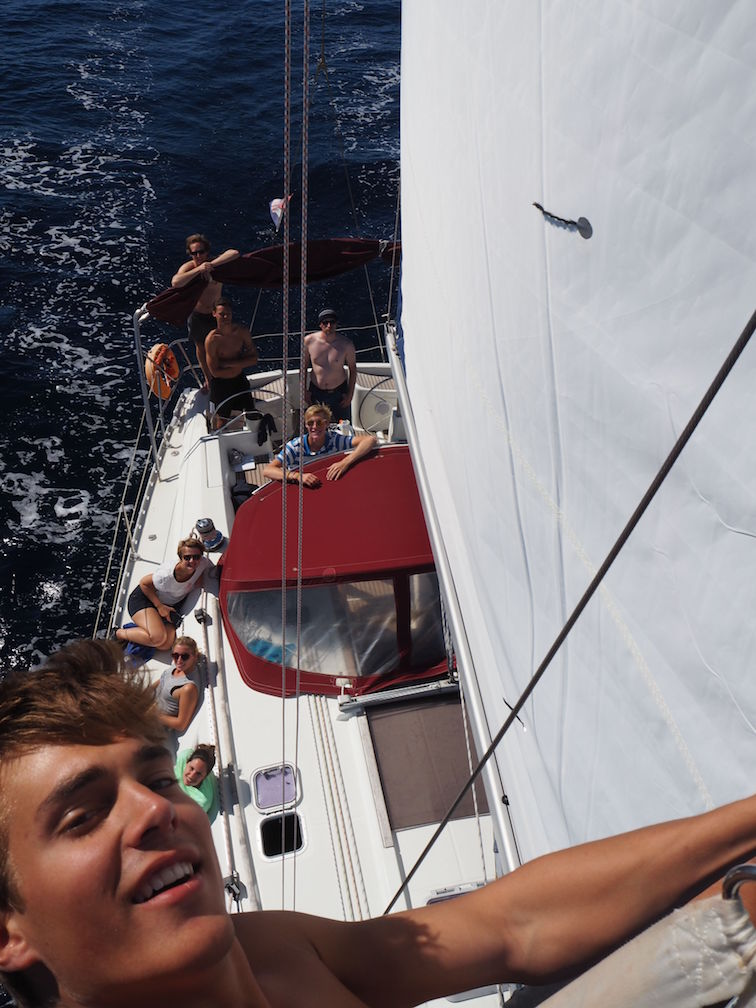
\includegraphics[width=0.435\textwidth]{rohmaterial-bilder/segeln.jpg}
    \end{center}
    \caption[Segeltörn mit dem USCU]{Segeln ist ein \glq wissenschaftlicher Sport\grq.}
  \end{wrapfigure}

Universitätspräsident Professor Michael Weber lobte in seinem Grußwort die außergewöhnliche Nachwuchsarbeit und dankte dem Verein für dessen erfolgreiche Außenwerbung. \glqq Segeln ist ein sehr wissenschaftlicher Sport. Hier kommen Leben, Lernen und Forschen zusammen\grqq, betonte der Präsident. Außerdem fördere das Segeln - wie von Hoppe bereits erwähnt - die Entwicklung persönlicher Fähigkeiten, darunter gerade auch solche, die in der Wissenschaft wichtig seien wie Mut, Ausdauer und Problemlösungskompetenz. 

Bei der Feier präsentierte sich auch der Shanty-Chor des USCU mit traditionellen Seemannsliedern, ganz klassisch begleitet mit Gitarre und Akkordeon. Und wie es sich laut Satzung für die „Commodores“ gehört, kamen die langjährigen ehemaligen Vereinsvorsitzenden Dr. Klaus Murmann und Professor Harald Traue ihren Repräsentationspflichten nach. Murmann, der gebürtige Füssener, der als Mitarbeiter in der Servicegruppe Informatik arbeitet, ist seit 1977 im Verein und übernahm gleich im ersten Jahr Verantwortung als Vorsitzender. Anekdotenreich rollte er in seiner Rede Seemannsgarn aus der Vereinsgeschichte auf und wusste vor allem von den Ausbildungstörns viel Amüsantes zu berichten. 

Harald Traue, der bis zu diesem Jahr als Professor die Sektion für Medizinische Psychologie leitete, kam 1989 zum USCU und war dreiundzwanzig Jahre lang Vorsitzender des Vereins. Der Wissenschaftler widmete sich in seiner Rede der anthropologischen und psychologischen Bedeutung des Segelns. Warum begibt man sich als Mensch ohne Not und Notwendigkeit auf das Wasser? Überflüssig, anstrengend und meistens dazu nass und kalt sei diese Tätigkeit. Traue sprach von den „healthy pleasures“, also vom gesunden Vergnügen, und erklärte die Faszination Segeln mit etwas Urmenschlichem, nämlich der ungeheuren Lust, auf das bewegte Wasser zu schauen. Und noch ein fundamentales Bedürfnis stille der Segelverein: das Bedürfnis nach Zusammenhalt in einer selbstlosen Gemeinschaft. „Unser Universitätssegelclub ist kein Profitcenter, sondern eine Solidargemeinschaft, die auch den Charakter ihrer Mitglieder prägt“, so der Commodore. Das kann auch an einer Universität nicht schaden. 

\cref{cha:2} ist auszugsweise dem Artikel in \cite[S. 54--56]{uni-ulm-intern} entnommen. Wir danken der Pressestelle der Universität Ulm für die freundliche Genehmigung der Verwendung von Text und Bild.
Praxis zu Tabellen und Formeln

In Tabelle *** hier Verweis auf die untenstehende Tabelle einfügen *** ist eine über eine Seite hinausreichende Tabelle zu sehen. 

% hier die Tabelle einfügen und sie nah wie möglich am Ziel-PDF gestalten

Durchschnittsnoten: Für und Wider

Schulnotendurchschnitten sollte man skeptisch gegenüberstehen, insbesondere da sie ja als arithmetischer Mittelwert, also als Summe aller Werte geteilt durch ihre Anzahl errechnet werden:

% hier erste Formel einfügen; achten Sie auf die Ausrichtung der beiden Zeilen und die Art der Nummerierung

Warum?
% Setzen Sie in den foldenden Absätzen an den betreffenden Stellen die korrekten Anführungszeichen:
Schulnoten sollen die Schulleistung messen. Wir alle wissen, eine Eins ist besser als eine  Zwei; diese ist besser als eine  Drei etc.
Doch um WIEVIEL ist die eine Note besser resp. schlechter als eine andere? Es sind zunächst nur Aussagen auf dem Niveau einer Rangskala (besser, schlechter, ...). Die Zahlen könnten auch  Sieben,  Dreizehn,  Siebzehn etc. lauten ...
Die Verwendung des arithmischen Mittelwerts setzt aber ein metrisches Skalenniveau voraus, bei dem die Zahlen einen konkreten definierten Wert auf der Skala haben. Erst dann macht es Sinn, sie zu addieren und durch ihre Anzahl zu teilen.

Richtigerweise sollte man auf dem Rangskalenniveau den Median als Maß für die  zentrale Tendenz verwenden. Der Median ist definiert als mittlerer Wert in der nach Größe geordneten Reihe aller Messwerte. Bei einer ungeraden Anzahl von Messwerten gibt es diesen Wert in der Mitte direkt, bei einer geraden Anzahl von Messwerten gibt es zwei Werte in der Mitte, die dann, so die Definition des Medians, arithmetisch gemittelt werden: beide Werte werden addiert und durch zwei geteilt: 

% hier die zweite Formel einfügen, siehe Kursbegleitendes Skript

So schön es ist, jetzt zu wissen, wie es richtig geht - mit derartigen Fragestellungen sind Kultusminister und auch viele Lehrer wohl doch überfordert.
% hier weitere Kapitel einbinden

\appendix

\backmatter
% diese Quellen werden nicht im Text ausdrücklich zitiert, erscheinen aber im Literaturverzeichnis

% hier erfolgt die Ausgabe des Literaturverzeichnisses
\nocite{*}
\printbibliography

\listoffigures
\end{document}
